\documentclass[border=5pt,tikz]{standalone}
\usepackage{amsmath} % for \dfrac
\usepackage{physics}
\usepackage{tikz,pgfplots}
\pgfplotsset{compat=1.18}
%\usepackage[outline]{contour} % glow around text
\usetikzlibrary{arrows,arrows.meta}
\usetikzlibrary{decorations.markings}
\usetikzlibrary{hobby}
\usepgfplotslibrary{fillbetween}
\usepgfplotslibrary{groupplots}
\tikzset{>=latex} % for LaTeX arrow head
\usepackage{xcolor}

\begin{document}

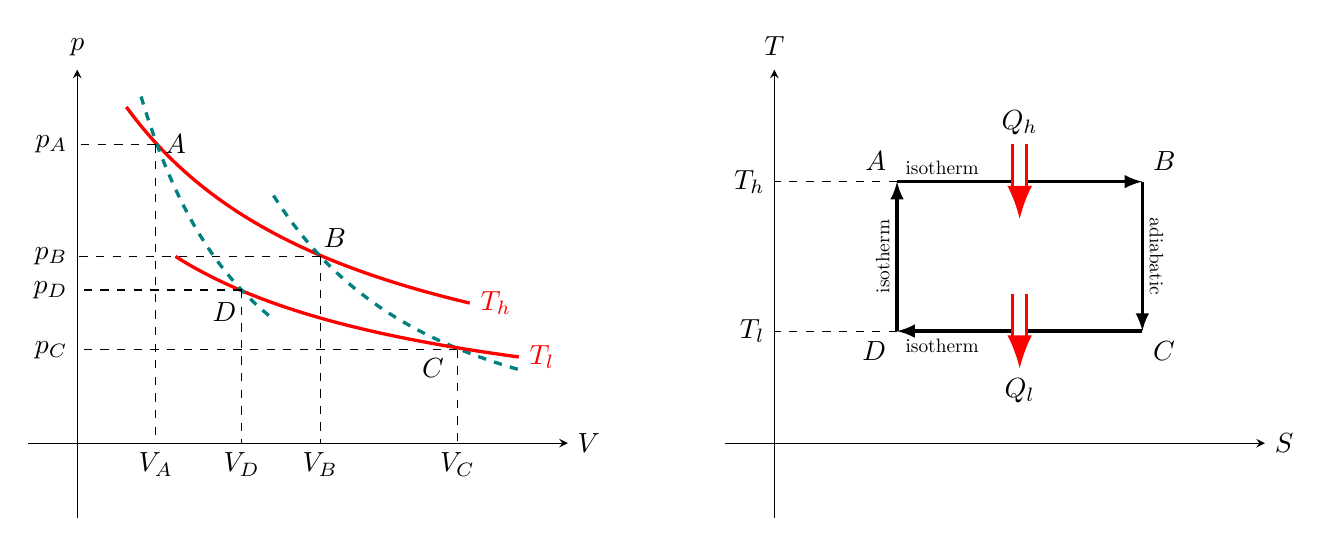
\begin{tikzpicture}
  \begin{groupplot}[
    group style={
        group name=plotGroup,
        group size=2 by 1,
        horizontal sep=2cm,
        vertical sep=1.5cm,
    },]
  \nextgroupplot[
  	axis lines=center,
    xlabel=$V$,
    ylabel=$p$,
    ticks=none,
    ymin = -2,
    ymax = 10,
    xmin = -2,
    xmax = 20.0,
    every axis x label/.style={at={(current axis.right of origin)},anchor=west},
    every axis y label/.style={at={(current axis.above origin)},above=0.5mm},
    ]
    \addplot [domain=5:12, samples = 100, very thick, red] ({(x-4)*2}, {45/x}) node[right] {$T_h$};
    \addplot [domain=8:13, samples = 100, very thick, teal, dashed] ({(x-4)*2}, {1200/(x^2.5)});
    \addplot [domain=6:13, samples = 100, very thick, red] ({(x-4)*2}, {30/x}) node[right] {$T_l$};
    \addplot [domain=5.3:8, samples = 100, very thick, teal, dashed] ({(x-4)*2}, {600/(x^2.5)});
    \node [] at (4, 8) {$A$};
    \node [] at (10.5, 5.5) {$B$};
    \node [] at (14.5, 2) {$C$};
    \node [] at (6, 3.5) {$D$};

    \def\Va{3.2};
    \def\Vb{9.9};
    \def\Vc{15.5};
    \def\Vd{6.7};
    \def\Pa{8};
    \def\Pb{5};
    \def\Pc{2.5};
    \def\Pd{4.1};
    \draw [dashed] ({\Va}, {\Pa}) -- (\Va, 0) node[below] {$V_A$};
    \draw [dashed] ({\Vb}, {\Pb}) -- (\Vb, 0) node[below] {$V_B$};
    \draw [dashed] ({\Vc}, {\Pc}) -- (\Vc, 0) node[below] {$V_C$};
    \draw [dashed] ({\Vd}, {\Pd}) -- (\Vd, 0) node[below] {$V_D$};
    \draw [dashed] ({\Va}, {\Pa}) -- (0, {\Pa}) node[left] {$p_A$};
    \draw [dashed] ({\Vb}, {\Pb}) -- (0, {\Pb}) node[left] {$p_B$};
    \draw [dashed] ({\Vc}, {\Pc}) -- (0, {\Pc}) node[left] {$p_C$};
    \draw [dashed] ({\Vd}, {\Pd}) -- (0, {\Pd}) node[left] {$p_D$};


    % \addplot [domain=1:19, samples = 100, thick, red] ({x}, {25/x});
    % \addplot [domain=0.3:19, samples = 100, thick, teal, dashed] ({x}, {55/(x^1.4)});
    % \legend{Isothermal, Adiabatic, ,};
     \nextgroupplot[
  	axis lines=center,
    xlabel=$S$,
    ylabel=$T$,
    ticks=none,
    ymin = -2,
    ymax = 10,
    xmin = -2,
    xmax = 20.0,
    every axis x label/.style={at={(current axis.right of origin)},anchor=west},
    every axis y label/.style={at={(current axis.above origin)},above=0.5mm},
    ]
    \addplot [very thick, -latex] (5, 7) -- node[above, scale=0.7, xshift=-4em] {isotherm} (15, 7) node [above right] {$B$};  
    \addplot [very thick, -latex] (15, 7) -- node[above, rotate=270, scale=0.7] {adiabatic} (15, 3) node [below right] {$C$};  
    \addplot [very thick, -latex] (15, 3) -- node[below, scale=0.7, xshift = -4em] {isotherm} (5, 3) node [below left] {$D$};  
   	\addplot [very thick, -latex] (5, 3) -- node[above, rotate=90, scale=0.7] {isotherm} (5, 7) node [above left] {$A$};  
 	\addplot [dashed] (5, 7) -- (0,7) node [left] {$T_h$};
	\addplot [dashed] (5, 3) -- (0,3) node [left] {$T_l$};
	\draw [red, line width=1pt, double distance=4pt,
             arrows = {-Latex[length=0pt 2 0]}] (axis cs:10,8) -- (axis cs:10,6);
	\node [above] at (axis cs:10,8) {$Q_h$};
	\draw [red, line width=1pt, double distance=4pt,
             arrows = {-Latex[length=0pt 2 0]}] (axis cs:10,4) -- (axis cs:10,2);
	\node [below] at (axis cs:10,2) {$Q_l$};
  \end{groupplot}

\end{tikzpicture}

\end{document}